%%%%%%%%%%%%%%%%%%%%%%%%%%%%%%%%%%%%%%%%%%%%%%%%%%%%%%%%%%%%%%%%%%
% Dokumentační část projektu do IMS.
% VUT FIT
% @author Josef Kolář, xkolar71
% @author Iva Kavánková, xkavan05
% @date 2018; 05; 12
%%%%%%%%%%%%%%%%%%%%%%%%%%%%%%%%%%%%%%%%%%%%%%%%%%%%%%%%%%%%%%%%%%

\documentclass[11pt, a4paper, titlepage]{article}

% Set document dimensions
\usepackage[paper=a4paper,top=1cm,left=2cm,right=2cm,bottom=2cm, includefoot]{geometry}
\usepackage{float}
\usepackage[final]{pdfpages} % inludesvg

% Czech fonts
\usepackage[T1]{fontenc}
\usepackage[utf8]{inputenc}
\usepackage[czech]{babel}
\usepackage{amsmath}
\usepackage{listings}
\usepackage{wrapfig}
% \usepackage{titlesec}
\usepackage{color} % barvy
\usepackage{xcolor} % vytváření barev
\usepackage{multicol}
\usepackage{newverbs}
\usepackage{lipsum}
\usepackage{svg}
\usepackage{gensymb}
\usepackage{caption}

%\usepackage{fancyhdr}

\usepackage{fancyhdr}
\usepackage{graphicx}


\lstnewenvironment{code}[1][]%
{\noindent\minipage{\linewidth}\lstset{frameround=fttf,#1}}%
{\endminipage}%

\definecolor{codeprimary}{HTML}{3300CC}
\colorlet{keywordstyle}{codeprimary!50!black}
\lstset{
language=C++,
frameround=fftf,
breaklines=true,
keywordstyle=\color{keywordstyle}\ttfamily,
basicstyle=\color{codeprimary},
numberstyle=\color{black},
backgroundcolor=\color{white},
frame=single,
tabsize=4,
breaklines=true,
captionpos=t,
xleftmargin=\dimexpr\fboxsep+1pt\relax,
xrightmargin=\fboxsep,
numbers=none,
showstringspaces=false,
escapeinside={\#!}{\^^M},
belowcaptionskip=0pt,
belowskip=0pt,
aboveskip=0pt,
}

\makeatletter
\newcommand\ic[1][green]{%
\@testopt{\@ic{#1}}{-#1}% Handle second optional argument
}
\def\@ic#1[#2]{%
\Collectverb{\@@ic{#1}{#2}}%
}
\def\@@ic#1#2#3{%
{\lstinline[basicstyle=\ttfamily\color{codeprimary},breaklines=true]|#3|}%
}
\newcommand{\icmacro}[1]{{\lstinline[basicstyle=\ttfamily\color{codeprimary},breaklines=true]|#1|}}
\makeatother


\setlength{\headheight}{3em}
\newcommand{\subsectionbreak}{\clearpage}

\begin{document}
    %%%%%%%%%%%%%%%%%%%%%%%%%%%%%%%%%%%%%%%%%%%%%%%%%%%%%%%%%%%%%%%%%%
% Dokumentační část projektu do IMS.
% VUT FIT
% @author Josef Kolář, xkolar71
% @author Iva Kavánková, xkavan05
% @date 2018; 05; 12
%%%%%%%%%%%%%%%%%%%%%%%%%%%%%%%%%%%%%%%%%%%%%%%%%%%%%%%%%%%%%%%%%%

\begin{titlepage}
    % \newgeometry{top=1in,top=2cm,left=2cm,right=2cm,bottom=2cm}

    \centering

    {\fontsize{20pt}{15pt}\bfseries
    VYSOKÉ UČENÍ TECHNICKÉ V~BRNĚ\\
    \vspace{8pt}
    Fakulta informačních technologií
    }

    
\includegraphics[scale=0.7]{./assets/fit-logo.pdf}

    \vspace{22pt}

    {\Large Modelování a simulace\\}
    \vspace{4pt}
    {\LARGE \bfseries Chov hmyzu pro potravinářské a průmyslové účely}

    \vspace{180pt}
    {\Large \today}

    \vspace{90pt}
    {\Large \bfseries Autoři\\}
    \vspace{12pt}

    \begin{tabular}{ l c r }
        Josef Kolář & \texttt{xkolar71} \\
        Iva Kavánková & \texttt{xkavan05} \\
    \end{tabular}\\

\end{titlepage}
    \pagestyle{fancy}
    \lfoot{\emph{VUT FIT - IMS}}
    \rfoot{\emph{Josef Kolář, Iva Kavánková}}
    \rhead{...}
    \lhead{Modelování a simulace}
    \tableofcontents
    \pagebreak
    %\noindent\makebox[\linewidth]{\rule{\textwidth}{0.4pt}}

    \section{Úvod}
    Tato práce vznikla jako projekt do předmětu Modelování a simulace. Zabývá se simulací (viz [\ref{ims}], slajd č. 8)
    modelu (viz [\ref{ims}], slajd č. 7) chovu cvrčků banánových (dále jen crvčci). Na základě daného modelu a sady simulačních experimentů (viz [\ref{ims}], slajd č. 33),
    bude ukázáno chování systému v rozdílných podmínkách. Smyslem projektu je demonstrovat, smysluplnost a finanční efektivitu hypotetické farmy na cvrčky.

    \subsection{Zdroje informací}
    Autoři projektu jsou Josef Kolář a Iva Kavánková. Při tvorbě došlo k čeprání znalostí z přednášek předmětu Modelování a simulace, z odborné literatury
    [\ref{kniha}], napsání dotazů na odborné internetové fórum (viz [\ref{forum}]) a taktéž od inženýrky Olgy Kavánkové, která je středoškolskou pedagožkou s aprobací na biologii
    a matematiku, čímž ji patří velké poděkování. Díky jejím odborným znalostem byl vytvořen odpovídající abstraktní model
    (viz [\ref{ims}], slajd č. 9).

    \subsection{Ověřování validity modelu}
    Validita (viz [\ref{ims}], slajd č. 37) byla ověřována při našem postupném testování. Výsledky byly porovnány s dříve získanými daty.
    Ověřování validity bylo považováno za úspěšné v momentě, kdy se výsledky simulace blížily s námi získanými informacemi.

    \section{Rozbor tématu a použitých metod/technologií}
    Pro modelování a simulaci hmyzí farmy je nutné znát její reálný chod. \\
    Životní cyklus cvrčka začíná jeho vylíhnutím, poté následuje týdenní doba, ve které vyroste a přes 90\% cvrčků je prodáno.
    Zbylí jedinci jsou ponecháni až do dospělosti (4 týdny od vylíhnutí). Samice po oplodnění samcem je schopna klást vajíčka, ze kterých vzniká
    nová generace. Nicméně, ne ze všech vajíček se narodí živí jedinci. Je také nutné brát v úvahu úbytek samců po soubojích, které provádí mezi sebou.
    Po týdnu kladení vajec samicemi, dojde k oddělení nakladených sít s vejcemi a vzniku nové generační nádoby (u chovu je to nutnost, neboť jinak dochází
    k obrovské míře kanibalismu). Zde nakladená vejce se po čase vylíhnou a cyklus pokračuje dál. Jelikož je samička plodná pouze určitou dobu,
    je poté prodána. Prodáni jsou také zbylí samci, neboť již dále by nepřinášeli žádný další zisk. Jelikože dospělí cvrčci jsou větší,
    vejde se jich do litru na prodej méně, než mladších cvrčků. Jedinci pochopitelně konzumují různé množství potravy podle svého věku. Crvčci potřebují k
    životu teplotu 28\degree C až 30 \degree C, tudíž je nutné výtápět jejich generační nádoby\\
    \\
    Shrnutí použitých číselných údajů pro model znázorňuje následující tabulka:

    \begin{table}[H]
        \begin{tabular}{|c|c|c|}

            \hline
            \textbf{Popis}                                         & \textbf{Hodnota}      & \textbf{Zdroj}                        \\ \hline
            Doba dospívání od vylíhnutí & (No) 4 týdny & Ing. Kavánková                   \\ \hline
            Doba, za kterou je jedinec vhodný k prodeji & (No) 1 týden & Převazato z [\ref{kniha}]             \\ \hline
            Množství denně nakladených vajíček & (No) 10 & Převazato z [\ref{kniha}]             \\ \hline
            Úspěšnost vylíhnutí jedince z vajíčka & 90 \%                 & Ing. Kavánková                   \\ \hline
            Doba od nakladení k vylíhnutí & (No) 2 týdny & Převazato z [\ref{kniha}]             \\ \hline
            Celková doba života jedince & (No) 12 týdnů & Ing. Kavánková                   \\ \hline
            Počet jedinců v 1 litru & 600 ks & Převazato z [\ref{forum}]             \\ \hline
            Počet nedospělých jedinců v 1 litru & 800 ks & Ing. Kavánková              \\ \hline
            Cena 1 litru jedinců k prodeji & 300 Kč & Průměrná hodnota z [\ref{cena}]       \\ \hline
            Denní úbytek samců po soubojích & 5 \%                  & Ing. Kavánková                   \\ \hline
            Denní množství potravy pro jedince starého 0 - 4 týdny & (No) 0,016 g & Převazato z [\ref{jidlo}]             \\ \hline
            Denní množství potravy pro jedince staršího 4 týdnů & (No) 0,034 g & Převazato z [\ref{jidlo}]             \\ \hline
            Cena 1 kg potravy & 800 Kč & Převazato z [\ref{forum}]             \\ \hline
            Vytápění pro 1 litr cvrčků & 12 W & Převazato z [\ref{topeni}]            \\ \hline
            Cena energie na 1 Wh & 1,2 Kč & Průměrná hodnota z [\ref{cena_topeni}]            \\ \hline
        \end{tabular}
        % \caption[Data]{Tabulka číselných údajů}
    \end{table}

    \subsection{Použité postupy}
    Program byl implementován v jazyce C++ s pomocí simulační knihovny SIMLIB (viz [\ref{simlib}]). To usnadňuje objektový návrh
    a třídy vhodné pro simulaci konkrétního zadání. Použité algoritmy byly použity ze slajdů k předmětu IMS (viz [\ref{ims}]), slajdy
    z prvního (viz [\ref{prvnidemo}]) a druhého (viz [\ref{druhedemo}]) demonstračního cvičení z tohoto předmětu.

    \section{Koncepce modelu}

    \subsection{Návrh konceptuálního modelu}

    \begin{figure}[H]
        \begin{center}
            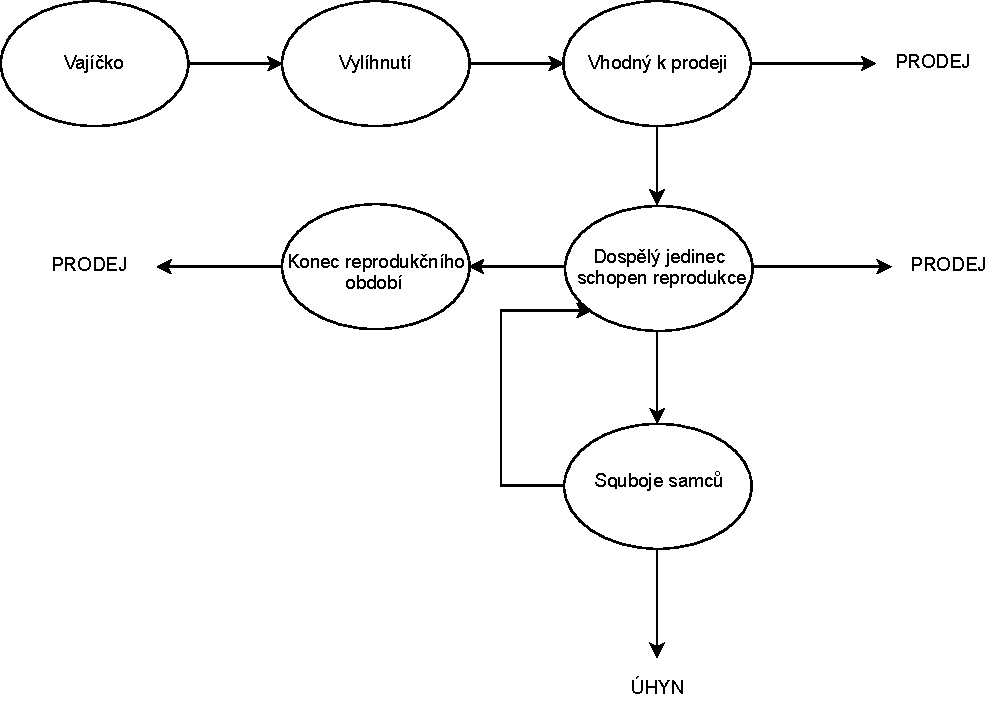
\includegraphics[width=.8\textwidth]{./assets/abstraktni_model.pdf}
            \caption{Abstraktní schéma}
        \end{center}
    \end{figure}

    \subsection{Formy konceptuálního modelu}

    \section{Architektura simulačního modelu}

    Simulační model využívá SIMLIB procesů reprezentujících jednotlivé jedince a jejich životní cyklus. Líhnutí vajíček
    je poté událost po vzoru SIMLIB a zajištuje vytvoření další procesů. Pro možnou analýzu rozložení generací
    jednotlivých jedinců v modelu je každému procesu přidělen atribut s pořadím generace. Pro agregaci těchto dat jsou
    použity nástroje ze simulační knihovny.

    \subsection{Rozbor implementace}

    Jádro simulační modelu leží ve třídách \ic|Cricket| a \ic|HatchEvent|. V případě první se jedná o proces modelující
    životní cyklus jednoho cvrčka, jakožto jedince. Druhá třída poté simuluje pomocí události nakladené vajíčko cvrčka -
    její naplánování do kalendáře zajištují samičky.

    \section{Podstata simulačních experimentů a jejich průběh}

    Pomocí experimentů nad modelem cvrččí farmy bychom rádi zoptimalizovali nastavení několika parametrů při jejím provozu
    vzhledem k ekonomice tohoto podniku. Jedná se o následující parametry:

    \begin{itemize}
        \item \textbf{Množství jedinců na počátku} - Množství přímo ovlivňuje další průběh provozu farmy, především rychlost
        jejího \uv{nastartování}, tedy odchování dostatečného počtu jedinců k založení další generace a prodeji.

        \item \textbf{Poměr jedinců k exportu} - Vzhledem k metodám chovu je nutno stanovit, jaké množství čerstvě
        vylíhnutých jedinců je určeno k exportu (a tím i jaké množství se následně množí a vytváří tak další generaci).
        Tento parametr je klíčový z hlediska udržení plné saturace farmy.

        \item \textbf{Kapacita farmy} - Farma jako taková má omezenou kapacitu kvůli užitým generačním nádobám. Vzhledem
        k realizaci modelu je tato hodnota pouze rámcová, nejedná se o pevný absolutní \uv{strop} pro počet jedinců.
    \end{itemize}

    \subsection{Postup experimentování}

    Při experimentování docházelo k úpravě výše uvedených parametrů, jednotlivé simulace byly prováděny na dvanáct měsíců
    a z výsledků simulace byly pozorovány následující metriky:

    \begin{itemize}
        \item \textbf{Počet jedinců v generaci} - Pomocí této metriky lze sledovat generační vývoj chovu, především
        jeho udržování v čase. Hodnota pro jednotlivou generaci velmi úzce souvisí s celkovou kapacitou farmy.
        \item \textbf{Počet jedinců prodaných pro nadbytek} - Touto metrikou lze pozorovat počet vylíhnutých cvrčků tzv. \uv{nadpočetně},
        tedy množství těch jedinců, kteří museli být prodáni kvůli omezené kapacitě farmy. Stejně jako předchozí metrika
        je závislý na celkové kapacitě, ale také především na poměru jedinců učených k exportu.
        \item \textbf{Finanční přehled běhu} - Ze zjištěných cen je spočítán finanční výsledek za simulované období.
        Na jedné straně se jedná o výdaje na počáteční generaci cvrčků, krmení a topení pro farmu - na druhé straně poté
        příjmy v podobě prodaných litrů cvrčků. Hlavním ukazatelem metriky je následně celkový hospodářský výsledek.
    \end{itemize}

    \subsection{Dokumentace jednotlivých experimentů}

    \subsubsection{Poměr jedinců k exportu}
    Cílem tohoto experimentu bylo nastavit parametr poměru exportu narozených cvrčků se stářím jeden týden tak, aby
    nedocházelo k extrémům ve velikosti populace.
    \begin{figure}[H]
        \centering
        \begin{minipage}{.48\textwidth}
            Pro velký poměr prodaných jedinců lze pozorovat postupné vyhynutí farmy (99 \% prodaných jedinců po narození):
            \begin{center}
                \begin{table}[H]
                    \begin{tabular}{|c|r|}
                        \hline
                        generace & počet \\
                        \hline
                        0. & 800  \\
                        1. & 11019  \\
                        2. & 1314  \\
                        3. & 284  \\
                        4. & 74  \\
                        5. & 47  \\
                        6. & 21  \\
                        7. & 0  \\
                        \hline
                    \end{tabular}
                \end{table}
            \end{center}
        \end{minipage}%
        \begin{minipage}{.5\textwidth}
            Pro nízký poměr lze pozorovat přebytky v generacích a tím i nutný prodej již narozené generace:
            \begin{center}
                \begin{table}[H]
                    \begin{tabular}{|r|r|r|}
                        \hline
                        generace & počet & přebytek \\
                        \hline
                        0. & 800 & 0 \\
                        1. & 11032 & 0 \\
                        2. & 138535 & 110219 \\
                        3. & 360772 & 331697 \\
                        4. & 365604 & 336787 \\
                        5. & 366491 & 336369 \\
                        6. & 239687 & 187799 \\
                        7. & 16546 & 7980 \\
                        \hline
                    \end{tabular}
                \end{table}
            \end{center}
        \end{minipage}
    \end{figure}
    \vspace{-20pt}
    \subsubsection{Kapacita farmy a celkový finanční výsledek}
    Při tomto experimentu bychom rádi potvrdili domněnku nevýhodnosti líhnutí nové generace v případě, že je farma
    kapacitně saturována a docházelo by tedy k přebytečnému stvoření nové generace.

    Pro počáteční generaci 800 jedinců (jeden litr mladých cvrčků) při kapacitě farmy 20 000 kusů jedinců a poměru exportu nově narozených cvrčků 90 \%
    je finanční výsledek za dobu simulace následující: \textit{(Dále budou prezentovány pouze celkové výsledky.)} \\
    \texttt{
        Sold: 130.097 l (appr. 39029 Kč)\\
        Feed: 21.1237 kg (appr. 16898 Kč)\\
        Power: 0.734442 WattDay (appr. 507 Kč)\\
        Total: 21324 Kč\\
    }

    Úpravou velikost počáteční generace lze částečně ovlivňovat roční výsledek farmy, je zde ovšem zásadně limitující
    kapacita farmy. Cvrčky lze považovat za tvory s vysokou reprodukcí, není tedy problém pro populaci za 1-2 generace
    saturovat farmu (při aktuálním měřítku). Při stejných parametrech je pro farmu s počátečním počtem cvrčků 16 000
    finanční výsledek \textbf{\texttt{Total: 23618 Kč}} - tedy nijak výrazný nárust zisku (oproti dvacetinásobné
    počáteční populaci).

    Za experimentování také stojí parametr udávající poměr exportovaných cvrčků týden po jejich vylíhnutí - především ve
    dvojici s parametrem pro kapacitu farmy - ten je pro tento experiment zvýšen na nedosažitelnou hodnotu, řádově $10^24$.
    S nastavením počáteční populace na 800 jedinců a poměru exportovaných mladých cvrčků na 25 \% je vidět exponenciální
    nárust počtu jedinců - z původních 800 je v šesté generaci přes 2'500'000 jedinců (800, 11'002, 38'931, 136'712,
    474'555, 1'653'306, 2'762'237). Zisk z této konfigurace farmy je neporovnatelný, ročně přesahuje 4'000'000 Kč. Na
    druhou stranu, podhodnocení tohoto má za následek vyhubení farmy, jak je vidět výše.

    \subsection{Závěry experimentů}

    Z provedených experimentů plynou jasné závěry:

    \begin{itemize}
        \item Díky vysoké reprodukční schopnosti je možné prodávat většinu cvrčků před dobou, než je schopen cvrček
        reprodukovat se, resp. není ekonomické cvrčka živit a poté prodat před dospělostí.
    \end{itemize}

    \section{Shrnutí simulačních experimentů a závěr}
    Jsme šikovní.

    \addcontentsline{toc}{section}{Reference}
    \begin{thebibliography}{zdroje}
        \bibitem{1} \label{ims} PERINGER P. Slajdy k přednáškám do předmětu Modelování a simulace, 2017. Verze 15. září 2017 [cit. 2018-12-05]
        \bibitem{2} \label{kniha} KOVAŘÍK, František. Hmyz: chov, morfologie. Jihlava: Madagaskar, 2000. ISBN 80-86068-24-2.
        \bibitem{3} \label{simlib} PERINGER P. Simulační knihovna SIMLIB pro C++, dostupné na https://www.fit.vutbr.cz/~peringer/SIMLIB/
        \bibitem{4} \label{prvnidemo} HRUBÝ M. Slajdy k I. democvičení, 2011 [cit. 2018-12-05]
        \bibitem{5} \label{druhedemo} HRUBÝ M. Slajdy k II. democvičení, 2011 [cit. 2018-12-05]
        \bibitem{6} \label{jidlo} [Online] http://www.openbugfarm.com/forum.html?fbclid=IwAR3tl0-KFHtvkUVEI5XdTn54CVVGcY5vnApXX0xmOnOQ5B78kurOgmtlcwo\#/discussion/1111/how-much-do-crickets-eat [cit. 2018-12-05]
        \bibitem{7} \label{forum} [Online] https://www.ifauna.cz/terarijni-zvirata/diskuse/detail/3524112/chov-cvrcku-v-cislech\#a3524888 [cit. 2018-12-05]
        \bibitem{8} \label{cena} [Online] https://www.broukarna.cz/cvrcci/cvrcek-bananovy-2-2/ [cit. 2018-12-05]
        \bibitem{9} \label{topeni} [Online] https://www.labet.cz/chov-krmneho-hmyzu-cvrcci-px1083117/ [cit. 2018-12-05]
        \bibitem{10} \label{cena_topeni} [Online] https://www.usetreno.cz/energie-elektrina/cena-elektriny/ [cit. 2018-12-05]
    \end{thebibliography}

\end{document}